\documentclass[]{tufte-book}

% ams
\usepackage{amssymb,amsmath}

\usepackage{ifxetex,ifluatex}
\usepackage{fixltx2e} % provides \textsubscript
\ifnum 0\ifxetex 1\fi\ifluatex 1\fi=0 % if pdftex
  \usepackage[T1]{fontenc}
  \usepackage[utf8]{inputenc}
\else % if luatex or xelatex
  \makeatletter
  \@ifpackageloaded{fontspec}{}{\usepackage{fontspec}}
  \makeatother
  \defaultfontfeatures{Ligatures=TeX,Scale=MatchLowercase}
  \makeatletter
  \@ifpackageloaded{soul}{
     \renewcommand\allcapsspacing[1]{{\addfontfeature{LetterSpace=15}#1}}
     \renewcommand\smallcapsspacing[1]{{\addfontfeature{LetterSpace=10}#1}}
   }{}
  \makeatother

\fi

% graphix
\usepackage{graphicx}
\setkeys{Gin}{width=\linewidth,totalheight=\textheight,keepaspectratio}

% booktabs
\usepackage{booktabs}

% url
\usepackage{url}

% hyperref
\usepackage{hyperref}

% units.
\usepackage{units}


\setcounter{secnumdepth}{2}

% citations
\usepackage{natbib}
\bibliographystyle{apalike}

% pandoc syntax highlighting
\usepackage{color}
\usepackage{fancyvrb}
\newcommand{\VerbBar}{|}
\newcommand{\VERB}{\Verb[commandchars=\\\{\}]}
\DefineVerbatimEnvironment{Highlighting}{Verbatim}{commandchars=\\\{\}}
% Add ',fontsize=\small' for more characters per line
\newenvironment{Shaded}{}{}
\newcommand{\AlertTok}[1]{\textcolor[rgb]{1.00,0.00,0.00}{\textbf{#1}}}
\newcommand{\AnnotationTok}[1]{\textcolor[rgb]{0.38,0.63,0.69}{\textbf{\textit{#1}}}}
\newcommand{\AttributeTok}[1]{\textcolor[rgb]{0.49,0.56,0.16}{#1}}
\newcommand{\BaseNTok}[1]{\textcolor[rgb]{0.25,0.63,0.44}{#1}}
\newcommand{\BuiltInTok}[1]{#1}
\newcommand{\CharTok}[1]{\textcolor[rgb]{0.25,0.44,0.63}{#1}}
\newcommand{\CommentTok}[1]{\textcolor[rgb]{0.38,0.63,0.69}{\textit{#1}}}
\newcommand{\CommentVarTok}[1]{\textcolor[rgb]{0.38,0.63,0.69}{\textbf{\textit{#1}}}}
\newcommand{\ConstantTok}[1]{\textcolor[rgb]{0.53,0.00,0.00}{#1}}
\newcommand{\ControlFlowTok}[1]{\textcolor[rgb]{0.00,0.44,0.13}{\textbf{#1}}}
\newcommand{\DataTypeTok}[1]{\textcolor[rgb]{0.56,0.13,0.00}{#1}}
\newcommand{\DecValTok}[1]{\textcolor[rgb]{0.25,0.63,0.44}{#1}}
\newcommand{\DocumentationTok}[1]{\textcolor[rgb]{0.73,0.13,0.13}{\textit{#1}}}
\newcommand{\ErrorTok}[1]{\textcolor[rgb]{1.00,0.00,0.00}{\textbf{#1}}}
\newcommand{\ExtensionTok}[1]{#1}
\newcommand{\FloatTok}[1]{\textcolor[rgb]{0.25,0.63,0.44}{#1}}
\newcommand{\FunctionTok}[1]{\textcolor[rgb]{0.02,0.16,0.49}{#1}}
\newcommand{\ImportTok}[1]{#1}
\newcommand{\InformationTok}[1]{\textcolor[rgb]{0.38,0.63,0.69}{\textbf{\textit{#1}}}}
\newcommand{\KeywordTok}[1]{\textcolor[rgb]{0.00,0.44,0.13}{\textbf{#1}}}
\newcommand{\NormalTok}[1]{#1}
\newcommand{\OperatorTok}[1]{\textcolor[rgb]{0.40,0.40,0.40}{#1}}
\newcommand{\OtherTok}[1]{\textcolor[rgb]{0.00,0.44,0.13}{#1}}
\newcommand{\PreprocessorTok}[1]{\textcolor[rgb]{0.74,0.48,0.00}{#1}}
\newcommand{\RegionMarkerTok}[1]{#1}
\newcommand{\SpecialCharTok}[1]{\textcolor[rgb]{0.25,0.44,0.63}{#1}}
\newcommand{\SpecialStringTok}[1]{\textcolor[rgb]{0.73,0.40,0.53}{#1}}
\newcommand{\StringTok}[1]{\textcolor[rgb]{0.25,0.44,0.63}{#1}}
\newcommand{\VariableTok}[1]{\textcolor[rgb]{0.10,0.09,0.49}{#1}}
\newcommand{\VerbatimStringTok}[1]{\textcolor[rgb]{0.25,0.44,0.63}{#1}}
\newcommand{\WarningTok}[1]{\textcolor[rgb]{0.38,0.63,0.69}{\textbf{\textit{#1}}}}

% longtable
\usepackage{longtable,booktabs}

% multiplecol
\usepackage{multicol}

% strikeout
\usepackage[normalem]{ulem}

% morefloats
\usepackage{morefloats}


% tightlist macro required by pandoc >= 1.14
\providecommand{\tightlist}{%
  \setlength{\itemsep}{0pt}\setlength{\parskip}{0pt}}

% title / author / date
\title{R for Environmental Health Research}
\author{Brooke Anderson}
\date{April 9, 2019}

\usepackage{booktabs}
\usepackage{amsthm}
\usepackage{fontspec}
    \setmainfont{Gill Sans}
\makeatletter
\def\thm@space@setup{%
  \thm@preskip=8pt plus 2pt minus 4pt
  \thm@postskip=\thm@preskip
}
\makeatother

\begin{document}

\maketitle



{
\setcounter{tocdepth}{1}
\tableofcontents
}

\hypertarget{prerequisites}{%
\chapter{Prerequisites}\label{prerequisites}}

\newthought{Based on requests from } some of the students for this
workshop, I've focused here on a few topics relevant to environmental health
research: organizing projects and tracking them with version control, creating
your own packages, and collecting and processing large datasets relevant to
environmental health research. You can download the slides from the workshop by
\href{https://github.com/geanders/columbia_env_health/raw/master/_workshop_slides/workshop_slides.pdf}{clicking
here}.

There are some additional topics in R that would also be useful for
environmental health researchers that I won't cover here. I would, however,
suggest that you look at the latest on tidyverse functions for cleaning and
visualizing data (the \texttt{dplyr} and \texttt{ggplot2} packages are at the heart of this),
new developments on working with geospatial data with the \texttt{sf} package, creating
interactive graphics with \texttt{htmlwidgets}, and creating reports, blogs, and books
through the \texttt{rmarkdown} framework. These are all areas for you to check out as you
continue developing how you use R for research.

Click on the \textbf{Next} button (or navigate using the
links at the top of the page) to continue.

\hypertarget{set-up}{%
\section{Set-up}\label{set-up}}

I am assuming that you already have R and RStudio installed on your computer.
You may want to check that you have a recent version of both, and if not, update
you version before the workshop. Some of the packages and RStudio tools we'll be
using will require newer versions of R and RStudio to work. You can run
\texttt{sessionInfo()} in R to find out the version of R you have installed. Compare
this version to the latest R release version listed at the Comprehensive R
Archive Network (CRAN).

To try out the examples, you will also need a bit more set-up:

\begin{enumerate}
\def\labelenumi{\arabic{enumi}.}
\tightlist
\item
  Download git
\item
  Get a GitHub account
\item
  Install some R packages
\item
  Download example R Project
\end{enumerate}

This section will walk you through each step.

\begin{enumerate}
\def\labelenumi{\arabic{enumi}.}
\tightlist
\item
  Download git
\end{enumerate}

In the workshop, you will learn how to use \textbf{git}.{[}\^{}\textbf{git.} Open-source version control
software that can be easily integrated with R projects.{]} To try the examples, you will need to
install git to your computer and make
sure that your installation of RStudio can find this software, so you can use git for version
control for R Projects. There are more details on this process in the ``Track'' section.

\begin{enumerate}
\def\labelenumi{\arabic{enumi}.}
\setcounter{enumi}{1}
\tightlist
\item
  Get a GitHub account
\end{enumerate}

You'll also learn how to share and collaborate on an R Project using \textbf{GitHub}.\footnote{\textbf{GitHub.}
  An online platform for directories tracked with
  the version control software \texttt{git}. This platform has become
  very popular for sharing code projects, as well as collaborating across a team on developing
  code and software. Other online git platforms exist and are used by some researchers,
  including \textbf{GitLab}. Once you've mastered using GitHub, you should be able to easy
  transfer those skills to other platforms like GitLab.} You will need to get a GitHub
account to be able to post repositories on GitHub.

\begin{enumerate}
\def\labelenumi{\arabic{enumi}.}
\setcounter{enumi}{2}
\tightlist
\item
  Install some R packages
\end{enumerate}

This booklet uses a number of R packages beyond base R. To install all the packages that you'll
need, run the following code in your version of R:

\begin{Shaded}
\begin{Highlighting}[]
\KeywordTok{install.packages}\NormalTok{(}\KeywordTok{c}\NormalTok{(}\StringTok{"devtools"}\NormalTok{, }\StringTok{"drat"}\NormalTok{, }\StringTok{"tigris"}\NormalTok{, }
    \StringTok{"ggplot2"}\NormalTok{))}
\end{Highlighting}
\end{Shaded}

Also, you'll want to install the \texttt{hurricaneexposuredata} and \texttt{hurricaneexposure} packages, which
you need to do in a bit of a different way:

\begin{Shaded}
\begin{Highlighting}[]
\KeywordTok{library}\NormalTok{(drat)}
\KeywordTok{addRepo}\NormalTok{(}\StringTok{"geanders"}\NormalTok{)}
\KeywordTok{install.packages}\NormalTok{(}\StringTok{"hurricaneexposuredata"}\NormalTok{)}
\KeywordTok{install.packages}\NormalTok{(}\StringTok{"hurricaneexposure"}\NormalTok{)}
\end{Highlighting}
\end{Shaded}

\begin{enumerate}
\def\labelenumi{\arabic{enumi}.}
\setcounter{enumi}{3}
\tightlist
\item
  Download example R Project
\end{enumerate}

I've created a repository on GitHub. You can find this example
repository by \href{https://github.com/geanders/columbia_env_health_examples}{clicking here}. On the
page takes you to, click on the ``Clone or download'' button and then select ``Download ZIP''.

This will download a single zipped file to your computer. When you unzip the file, it will be a
special type of directory, an R Project directory. To open the R Project and start on the
examples, open RStudio, then go to ``File'' -\textgreater{} ``Open Project''. A pop-up window will open to let you
navigate through your files and find an R Project to open. Navigate to the directory you
downloaded, which should be called ``columbia\_env\_health\_examples'' and doubleclick on the file
in this directory called ``columbia\_env\_health\_examples.Rproj''.

This will open the project. In the ``Files'' pane of RStudio, you should see some subdirectories for
``R'' and ``data''. These have the example R code and data, respectively, for you to try the examples
in this booklet. The code in each of the R files should run independently, including the code to
load all required packages. Figure \ref{fig:examplerepo} shows what this package should
look like once you've downloaded and opened it, as well as some of the files in the
project's ``R'' subdirectory.

\begin{figure*}
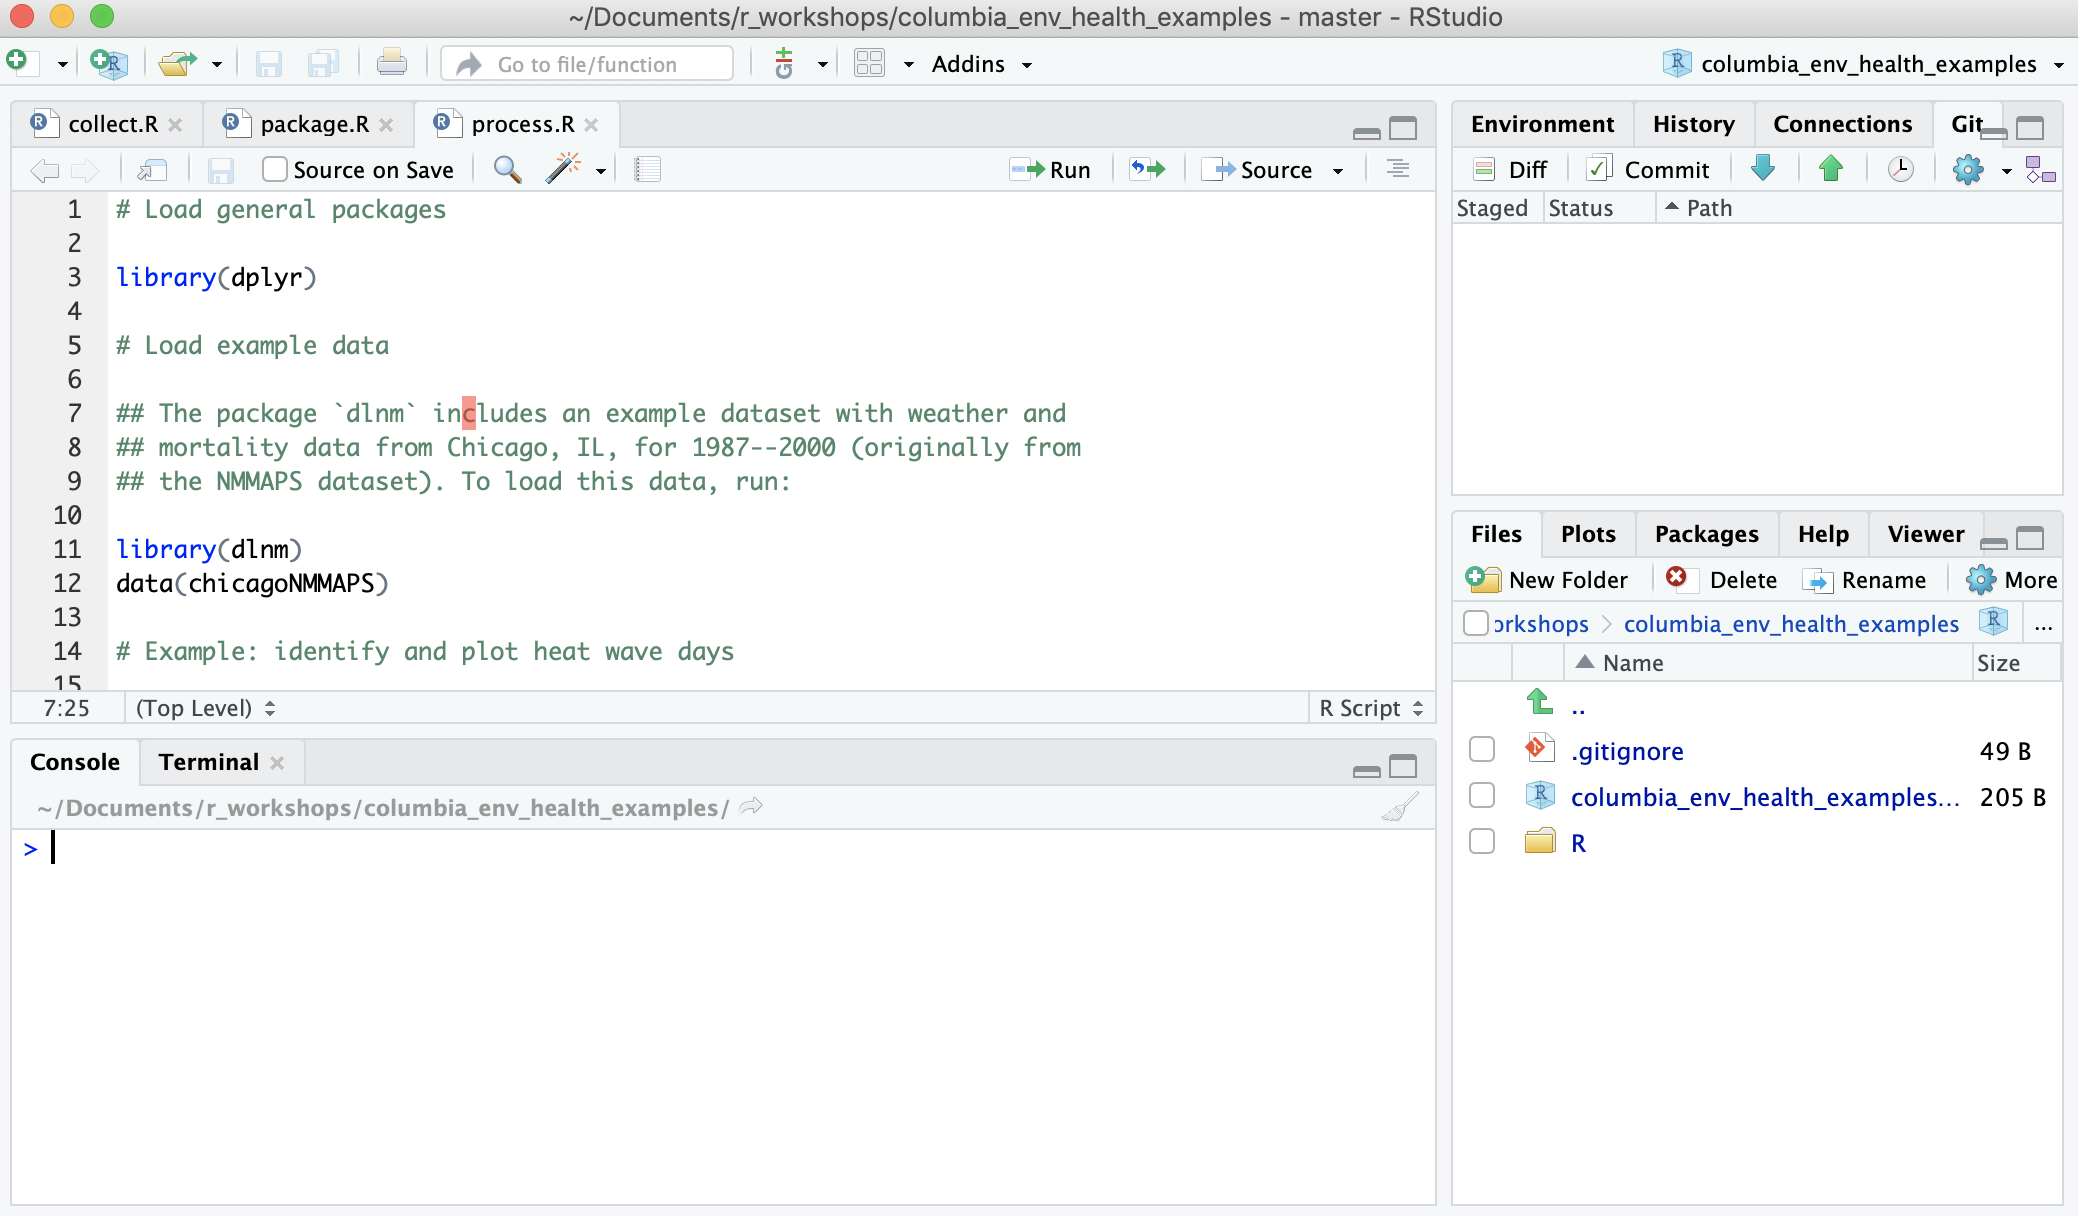
\includegraphics[width=28.86in]{images/example_repo} \caption[What the example R Project for this booklet should look like once you've downloaded and opened it]{What the example R Project for this booklet should look like once you've downloaded and opened it.}\label{fig:examplerepo}
\end{figure*}

\hypertarget{organize}{%
\chapter{Organize}\label{organize}}

\newthought{If you are using R to write} for larger projects, including
research for academic papers and theses, you should start putting some thought
into how you organize your research files, including raw data, cleaned data,
coding scripts for analysis, and output like paper drafts and figures. So far,
you may have run much of your analysis within a single R script or R Markdown
file. Often, any associated data are within the same working directory as your
script or R Markdown file, but the files for one project are not separated from
files for other projects. As you move to larger projects, this kind of set-up
won't work as well. Instead, you'll want to start keeping all materials for a
project in a single and exclusive directory.

\hypertarget{r-projects}{%
\section{R Projects}\label{r-projects}}

\newthought{RStudio allows you to} create ``Projects'', which help with this
organization. An R Project is very simple---it's just a file directory, with an
extra subdirectory added to the directory with settings to remind RStudio about for the project. This directory is
saved as a dot file, so you probably won't be able to see it
listed if you look at the directory contents using your computer's file finder. If you'd like
to see the listing (or delete it by hand, although you likely won't ever need to
do this), check the settings for your file finder, and see if you have the option
to show all files. Alternatively, you can use the ``list'' command with the ``all'' option
(\texttt{ls\ -a}) at a Bash shell to view all files and subdirectories in a directory.

Advantages of setting a directory to be an R Project are:

\begin{itemize}
\tightlist
\item
  Automatically uses the directory as your current working directory when you open the project.
\item
  Coordinates well with git version control and GitHub repository system.
\item
  Opens a ``Files'' window for navigating project files in an RStudio pane when you open the project.
\end{itemize}

You can either create an R Project as a new directory or convert an existing directory into
an R Project. To do either, in RStudio go to the ``File'' menu and select ``New Project''. You'll
then have the option to either create a new directory that's an R Project or to search through
your computer's files to find an existing directory to make into an R Project.

Once you've created an R Project, you can open it in RStudio; opening an R Project will set
the project's directory as your working directory, opening a ``Files'' window with all the
subdirectories and files in the project directory and allowing you to run code with
relative filenames from the project's directory. If you
share the R Project with someone else,\footnote{One way to do this would be to zipped the directory
  into a single file and share it by email. Another is to use git version control, post the
  directory to GitHub, and share the directory from there.} he or she will also be able to
open the R project using RStudio.

One benefit of R Projects is that it is very easy to initialize them as git repositories.
A later section (``Track'') will go over how to initialize and use git version control for
R Projects. You will also definitely want to use an R Project for any R package you write,
as this will introduce a lot of functionality that ``plays well'' with the \texttt{devtools} package
to make it easier to write, build, and publish an R package.

\hypertarget{directory-organization}{%
\section{Directory organization}\label{directory-organization}}

My desk at work is very messy, with lots of paper printouts piled up. But I do
keep my project directories very tidy, and I strongly recommend the practice.

This goes beyond ``well-organized'', which we just covered (putting all project
files in one directory, using subdirectories to divide up files in a project,
using consistent names for project file directories, etc.). Keeping a project
directory ``tidy'' means having \textbf{only one} version of each file. Often, as you
develop a project, especially when collaborators are involved, you can end up
with many versions of a file. For example, you may have the draft of a journal
article's text saved in some versions with the file name reflecting the date of
the draft (``draft\_may\_12.docx''), some versions that include the initials of
people who reviewed it (``paper\_draft\_ba\_rp\_mb2.docx''), and so on.

This type of organization---having multiple versions of project files, with the
file names meant to help you keep track of them---results in very cluttered and
hard-to-manage project directories. Instead, at any given moment, each of your
project directories should have only one version of each project file. You
certainly won't want to lose information from edits and changes to the files
along the way, so it's smart to use some type of \textbf{version control
system}{[}\textbf{version control system.} Software for tracking changes to software
projects. Some researchers who use a lot of coding also use this software to
track their projects One well-known example is \textbf{git}, but there are other
version control systems as well.{]} on each project directory. This will allow you
to track the changes you've made to each file and to go back and revisit the
file at any moment in the project's history. A later section of this booklet
(``Track'') will describe how you can use \texttt{git} for version control for R
projects.

\hypertarget{avoiding-repetition}{%
\subsection{Avoiding repetition}\label{avoiding-repetition}}

One key to efficient organization is to \textbf{avoid repetition}.\footnote{In programming,
  you'll often hear this advice as ``Do Not Repeat Yourself''.} In practice, it
often happens that you're using the same code across several projects. For
example, say you have some code that calculates the apparent temperature from
air temperature and some measure of dewpoint temperature. If you have organized
your project files to have one directory per paper, with all the associated code
for a paper within the project's directory, then you may find you're often
copying and pasting the code to calculate apparent temperature into different
directories.

This situation makes for a tricky balance---you want to organize your files and
have a separate directory for each project, but cutting and pasting code can be
a recide for disaster. Each time you move the code, there's a chance for an
error to slip in. Also, what if you want to make a change in the code? Say you
hear about a better algorithm for calculating apparent temperature? You will
either need to go through all of your projects that use that code and change the
code everywhere, or you will have to settle for different projects using
different algorithms.

This means it's time to start thinking about writing your own R package. You do
not have to publish every R package you write---it's fine to just use it
yourself and not share it more widely. Regardless, a package is the right place
to store related code that you use often, as well as documentation (and possibly
tests) to go with that code. A later section of this booklet (``Package'') will go
over a bit about how to write your own R packages, as well as references for
learning more about package development.

\hypertarget{learn-more}{%
\section{Learn more}\label{learn-more}}

\href{https://www.amazon.com/Reproducible-Research-Studio-Chapman-Hall/dp/1466572841}{Reproducible Research with R and R Studio} is an excellent book with advice on improving the reproducibility of
projects using R, including academic research projects.

A few good articles have come out recently that describe project organization within
different scientific fields (e.g., biology, archaeology, ecology).
It's worth searching Google Scholar for ``reproducible research in R'' and your own
or a closely related research field.

\hypertarget{package}{%
\chapter{Package}\label{package}}

\newthought{As with many other things in R,} the threshold of complexity
for writing your own package has recently lowered dramatically. If you are writing
some of your own functions in R to use for your research, and you've become comfortable
with writing functions, you should try putting them in an R package. You don't have
to share this package through publishing it on CRAN or another repository---instead, it's
fine to start by just writing packages for your own use, or for your research group's
private use. However, once you start writing packages, you will see how straightforward
it is, and you may want to take the extra steps to prepare your package for CRAN and
submit it.

An R package is just ``a directory of files which extend R'' (\url{https://cran.r-project.org/doc/manuals/r-release/R-exts.html}).
You should consider writing your own package anytime you find yourself cutting and pasting
functions to different directories on your computer, so you can use them for different
projects. The RStudio team has created a number of tools to make this process easier, including
some functionality in the RStudio IDE as well as the \texttt{devtools} package \citep{R-devtools}.

\hypertarget{components-of-r-packages}{%
\section{Components of R packages}\label{components-of-r-packages}}

\hypertarget{r-code}{%
\subsection{R code}\label{r-code}}

Without R code, there's not much point to an R package.\footnote{The exception? A data-only package,
  where the package's purpose is to share data rather than R functions. We'll look at an
  example in the ``Collect'' section.} The R function code will go in the package's ``R''
subdirectory. You can use as many or as few ``.R'' files in this section as you want to
organize your code.
Define your functions in this section as you would if you were creating functions in
an R script. As you become more advanced in writing packages, you may want to start
adapting your function code a bit. For example, the \texttt{package::function} notation can
help keep clear which package you mean for a function to call a function from, and so
the behavior will be stable regardless of the order that a user loaded packages.
Also, if you intend for your functions to be used inside tidyverse pipelines, you'll
want to take a look at the developing \href{https://tidyeval.tidyverse.org/}{Tidy evaluation} book.

Although it is not required for a package you're creating just to use yourself, you
should think about adding help documentation to your code very early. You can then
access this documentation through helpfiles in R, just like you do with other R packages.
Even if you are just creating a package for yourself, you should add documentation
for all the ``top-level'' functions\footnote{\textbf{top-level functions.} The functions in your package
  that you expect your users (including yourself) to call directly. Your package may also
  include some functions that are ``helpers'', only used within other functions to help
  keep the code clean and avoid replication, but never used directly by package users.}

Years ago, you would need to write this documentation in separate ``.Rd'' files
and save them in the ``man'' subdirectory. Now, the easiest thing to do is to use
``roxygen'' conventions to write the help information right above each function.
With this style, you'll use a special type of commenting character (\texttt{\#\textquotesingle{}}) at the
start of each line with documentation, and there are special codes (e.g.,
\texttt{@param} when you're defining one of the function's parameters) to annotate this
code. This help documentation will then, when you build your package, be
converted to the ``.Rd'' files you used to have to write yourself and saved in the
``man'' directory. Several of the resources listed in ``Learn more'' give more
details on writing and rendering this help documentation.

\hypertarget{description-file}{%
\subsection{DESCRIPTION file}\label{description-file}}

Every package directory must have a DESCRIPTION file, but if you aren't sharing
the package, there's no harm in leaving this as the original template file you
get when you start a package directory using RStudio (you'll try this out in
just a minute). The exception is when your functions rely on functions from
other R packages---in this case, you'll want to add in these dependencies in the
DESCRIPTION file. That way, when you load your package, all of these will also
be loaded.

If you plan to share your package with others, however, and especially if you
plan to publish your package in CRAN or another repository, you'll need to do
a lot more with the DESCRIPTION file. This file provides the metadata on your package,
including the authors, version, description, and dependencies on other packages.
The \textbf{R Packages} book referenced in the ``Learn More'' section has extensive advice
on editing this file for packages meant for publication.

\hypertarget{other-package-components}{%
\subsection{Other package components}\label{other-package-components}}

So far, I've described the barebones elements you'll need to have to create a very
minimalist package. There are, however, a number of other elements you'll often
want to add to the package. As with the R code for package functions and the
DESCRIPTION file, there is a specific location and format required for each of
these elements within an R package.

Some of the most common components you'll want to add include example datasets
(which will go in a \texttt{data} subdirectory), tutorials for using the package
(\texttt{vignettes} subdirectory), and unit tests for the functions (\texttt{tests}
subdirectory). To help you set up these extra components, you may want to take a
look at the \texttt{use\_*} family of functions in the \texttt{usethis} \citep{R-usethis}
package\footnote{The \texttt{use\_*} family of functions were previously in the \texttt{devtools}
  package, but they are being deprecated there and moved to the \texttt{usethis} package.
  The \href{http://r-pkgs.had.co.nz/}{R Packages} book was written before they were
  deprecated in \texttt{devtools}, and so it discusses them as \texttt{devtools} functions. As
  long as you install and load the \texttt{usethis} package, though, you'll have no
  problem following along with the examples in that book.} For example, if you
want to include example data in your package, you should check out the
\texttt{use\_data} function, while if you want to add unit tests to your package, check
out the \texttt{use\_test} function. When you run one of these, you'll notice that the
function \emph{adds files and subdirectories} when needed to your R package
directory. This may throw you at first, since most R functions don't make
changes to your file directory, but you'll need those added files to add the
package components, and it's \emph{much} easier to remember a single function call to
run when you need to add one than to remember all the details of which files (and
in what structure) need to be added.

\hypertarget{try-it-out}{%
\section{Try it out}\label{try-it-out}}

I suggest you try out the following steps to experiment with
writing your own package. I've included a function for you to build
your package around in the ``package.R'' file of the R project with
examples for the workshop.

\begin{itemize}
\tightlist
\item
  Create a new R Project for your R package
\item
  Build the package
\item
  Move a function into the right place in the package
\item
  Edit the DESCRIPTION file as needed
\item
  Add example data into the right place in the package
\item
  Add some unit tests for the function
\item
  Add documentation using roxygen2 notation
\item
  Add a short vignette
\end{itemize}

I'll walk you through the first three steps, and then I suggest you use
Hadley Wickham's \textbf{R Packages} book (see the ``Learn More'' section) to
get some tips as you try out the rest on your own.

\textbf{Create a new R Project for an R package.} Open RStudio and go to ``File'' -\textgreater{}
``New Project''. Choose ``New Directory'' and then ``R Package''. Name your package
``convertr''. Then click on ``Create Project''.

The R Project you've just created will open in RStudio. If you look in the ``R''
subdirectory, you'll see there's one file called ``hello.R''. There's also a
subdirectory called ``man''and three files in the top directory called
``.Rbuildignore'', ``DESCRIPTION'', and ``NAMESPACE''.

\textbf{Build the package.} This project opens with a template---a very small but working package that can
serve as a skeleton as you adapt the files to create your own package. Before you
do anything to change from the template, try building the package using the
\texttt{build} function from the \texttt{devtools} package:

\begin{Shaded}
\begin{Highlighting}[]
\KeywordTok{library}\NormalTok{(devtools)}
\KeywordTok{build}\NormalTok{()}
\end{Highlighting}
\end{Shaded}

You should get some output like this:

\begin{verbatim}
✔  checking for file ‘/Users/georgianaanderson/Documents/r_workshops/convertr/DESCRIPTION’ ...
─  preparing ‘convertr’:
✔  checking DESCRIPTION meta-information ...
─  checking for LF line-endings in source and make files and shell scripts
─  checking for empty or unneeded directories
─  building ‘convertr_0.1.0.tar.gz’
\end{verbatim}

Congratulations! You've built (maybe) your first R package. You should now be able to
load it like any other R package on computer and run its function. Try running:

\begin{Shaded}
\begin{Highlighting}[]
\KeywordTok{library}\NormalTok{(convertr)}
\KeywordTok{hello}\NormalTok{()}
\end{Highlighting}
\end{Shaded}

To build the package in a way that you can use it anywhere on your computer,
go to the ``Build'' tab in RStudio and click ``Install and Restart''. As long
as you don't get warning messages, you should be able to load and use the
package from any R session on your computer.

\textbf{Move a function into the right place in the package.}

Now try adapting the template into your own package. Delete the file
``hello.R'' in the ``R'' subdirectory. Create a new file in this subdirectory
called something like ``temp\_conversions.R''. Copy the code for the
\texttt{c\_to\_f} function, which is in the ``package.R'' file of the R Project
with examples for this workshop. Save the file and rebuild the package,
either with the \texttt{build} call to build within that project or with the
``Install and Restart'' button in the ``Build'' tab to make it available
anywhere on your computer.

\hypertarget{sharing}{%
\section{Sharing}\label{sharing}}

\hypertarget{when-to-publish-your-packages}{%
\subsection{When to publish your packages}\label{when-to-publish-your-packages}}

Once you have some functions that you think others might find useful, you
should consider creating a package with them and sharing that package with
others. Similarly, if you have a dataset that you think others might
find useful and that you have permission to share, you should consider creating
a data-only package to use to share that data.

\hypertarget{where-to-publish-packages}{%
\subsection{Where to publish packages}\label{where-to-publish-packages}}

There are a few ways to publish your R package, and they have different
levels of requirements as well as different levels of recognition (including
for CVs and progress reports).

First, you can share the ``tar.gz'' file that's create when you run ``Install and Restart''
for an R package from RStudio. The other user can install this file locally using
\texttt{install.packages} with some extra options. For example, if you shared your
``convertr.tar.gz'' package file with someone else, they could install it on their
computer with the call:\footnote{This call assumes that the other person has ``convertr.tar.gz''
  saved in his or her working directory. Otherwise, use a pathname to direct R to where
  the file is saved on the computer.}

\begin{Shaded}
\begin{Highlighting}[]
\KeywordTok{install.packages}\NormalTok{(}\StringTok{"convertr.tar.gz"}\NormalTok{, }\DataTypeTok{repos =} \OtherTok{NULL}\NormalTok{, }
    \DataTypeTok{type =} \StringTok{"source"}\NormalTok{)}
\end{Highlighting}
\end{Shaded}

Second, and perhaps even easier (certainly for the other user), you can post your
package as a GitHub repository. The other user can then use the \texttt{install\_github}
function from the \texttt{devtools} package to install the package. Unless you set
the repository to be private, be aware that your package code would be public.
This means anyone could install and use it, although if you don't publicize it,
it's unlikely that many people will.

If you want to share your package more widely, you should submit it to a repository.
The \href{https://cran.rstudio.com/}{Comprehensive R Archive Network (CRAN)} is the most
popular for most scientific fields. The \texttt{devtools} package has some tools specifically
for checking and releasing a package to CRAN. \href{https://www.bioconductor.org/}{Bioconductor}
is the top choice for many bioinformatics packages.

Finally, an excellent choice is to submit the package to
\href{https://ropensci.org/}{ROpenSci} for peer review. If you are thinking of doing this,
check ROpenSci's policies on what types of packages are considered ``in scope'' for it.
If you submit a package here, it will be openly reviewed by two other R programmers,
with an open review process. You will then have the chance to revise the package
code in response to the reviewers' comments. Accepted packages can also be
submitted to CRAN or Bioconductor.

\hypertarget{extra-steps-for-publishing}{%
\subsection{Extra steps for publishing}\label{extra-steps-for-publishing}}

If you want to submit your package to CRAN, you'll need to take a few extra
steps to get it ready. These steps aren't necessary for a package you plan to
just use privately, but they wouldn't be a bad idea to try to do even in that
case. For example, you'll need to make sure that the functions in your package
are comprehensively documented. Every function that you expect an end user might
use should have a helpfile. In addition to documenting specific functions, you
should also consider writing overall tutorials (called \textbf{vignettes}) that walk
a user through how to use your package in a few example scenarios. You will also
need to make sure that your package can run on different operating systems. If
your package only has straightforward functions written exclusively in R, with
little interaction outside of R on the user's computer, this shouldn't be an
issue. However, you should still check before submitting to CRAN. Several of the
resources listed in ``Learn More'' have very detailed information on preparing a
package to submit to a public repository.

\hypertarget{learn-more-1}{%
\section{Learn more}\label{learn-more-1}}

One wonderful resource for writing and publishing R packages is the book \href{http://r-pkgs.had.co.nz/}{R
Packages} by Hadley Wickham \citep{wickham2015r}. This book
is available for a reasonable price in paperback (many Barnes \& Nobles carry it
in their computer section) and is also available for free online. The author of
this book also created and maintains the \textbf{\texttt{devtools} package}\footnote{\textbf{\texttt{devtools}
  package.} An R package with functions that facilitate R package development.
  These functions are well-documented in the package documentation as well as
  through the book \href{http://r-pkgs.had.co.nz/}{R Packages}. This package also
  includes a function for installing R packages from code posted on GitHub
  (\texttt{install\_github}), which is very useful if you want to find and use packages
  that are not yet available on CRAN and other repositories or if you want to use
  the latest, ``development'' version of a package. This package is available on
  CRAN and so can be installed with \texttt{install.packages("devtools")}.} The ``Package
Development'' cheatsheet available through \href{https://www.rstudio.com/resources/cheatsheets/}{RStudio's
cheatsheets} complements these
resources.

Along with Roger Peng and Sean Kross, I co-teach a Coursera Specialization on
\href{https://www.coursera.org/specializations/r}{Mastering Software Development in
R}, and we also have \href{https://bookdown.org/rdpeng/RProgDA/}{an online
book} on bookdown on the topic. The
official CRAN resource for writing packages, \href{https://cran.r-project.org/doc/manuals/r-release/R-exts.html}{``Writing R
Extensions''}, is
available online. However, it gets very technical, and so I recommend starting
with other resources and working up to this document.

To learn more about best practices for creating R, especially for publication,
check out \href{https://ropensci.github.io/dev_guide/}{ROpenSci's handbook}. ROpenSci
conducts peer review for R packages, and it's all conducted openly. You can
learn a lot about packages and package development, especially for more complex
packages, by following this peer review package. It's all conducted through \href{https://github.com/ropensci/software-review/issues}{the
``Issues'' in a GitHub repo}.

If you end up writing and publishing a lot of R packages through your scientific
research, you may find that you need to help your supervisors and peers
understand this research project. One recent article discusses how academic
research in the data science realm is changing, as well as how department chairs
and others can evaluate these new research products, including for promotion and
tenure \citep{waller2018documenting}.

\hypertarget{track}{%
\chapter{Track}\label{track}}

\newthought{Years ago, I tried to learn to use} git version control software with R, and
it was a total fail. Maybe it's just me, but I found it really hard to wrap my head around
the text-dominated, command-line interface classically used for git. However, RStudio now
includes tools that provide a GUI-style
interface to most of the functionality you'll need from git for R-based projects. I highly
recommend trying git by using it through RStudio first, and then once you develop a mental
map of what's going on, it's much easier to transfer partially or completely to running git
from a shell.

In this part, I'll discuss both git (the software that allows you to track changes to your
R projects), as well as GitHub (an online platform for sharing and collaborating on
version-controlled projects). I'll also discuss, near the end, how to use either a Bash
Shell or the \texttt{git2r} package to do some one-off git tasks that can't be done directly through
the RStudio GUI-style git interface.

\hypertarget{git}{%
\section{git}\label{git}}

Git is a version control system. It saves information about all changes you make
on all files in a repository. This allows you to revert back to previous
versions and search through the history for all files in the repository. Git is
open source. You can download it for different operating systems at
\url{https://git-scm.com/downloads}. You will need git on your computer to use git
with RStudio and create local git repositories you can sync with GitHub
repositories. If you are using Windows OS, you'll want your git installation to
include a ``Bash emulation'' (i.e., access to a command line that acts like a Bash
shell), which I think should come standard with the Windows git installation.
On Mac or Linux computers, you should already have access to a Bash shell.

\hypertarget{configuring-git}{%
\subsection{Configuring git}\label{configuring-git}}

Before you use git, you should configure it. For example, you should make sure
it has your name and email address. You can configure git with commands at a
Bash shell.\footnote{If you are using Windows, search for ``Bash'' among your programs.
  You should be able to fine the Bash emulator that cam with your git install. If
  you are using a Mac, you'll want to open ``Terminal''. If you're using Linux, you
  almost certainly already know your way around a Bash shell.} For example, I
would run the following code at a shell to configure git to have my proper user
name and email:

\begin{verbatim}
git config --global user.name "Brooke Anderson"
git config --global user.email "brooke.anderson@colostate.edu"
\end{verbatim}

You'll only need to run this configuration once, until you get a new computer or
for some reason need to re-install git. Once you set these configurations on
your computer, they should be set on that computer indefinitely.

Next, you need to make sure that RStudio can find the git software you
installed. Sometimes, RStudio will automatically find git (once you've installed
git) when you start RStudio. However, in some cases, you may need to take some
more steps to activate git in RStudio. To do this, go to ``RStudio'' -\textgreater{}
``Preferences'' -\textgreater{} ``Git/SVN''. Choose ``Enable version control''. If you have just
installed git, and have not restarted RStudio, you'll need to do that before
RStudio will recognize git. If you do not see ``Git'' in the box for ``Version
control system'', it means either that you do not have git installed on your
computer or that RStudio was unable to find it. If RStudio doesn't find your
version of git in the ``Git executable'' box, browse for it. If you're still
having problems, there's a chance that you'll need to mess around some with your
PATH variables. You may want to find a computer-savy friend or IT person to help
you if you get to this stage.

\hypertarget{tracking-an-r-project}{%
\subsection{Tracking an R project}\label{tracking-an-r-project}}

To track an R package, you'll first need to initialize it as a git repository.
Then, as you make changes to the code, you'll want to \textbf{commit} those changes
as you go, using \textbf{commit messages} that are short but clear enough for you to
follow them when you review them later.

You can initialize a git repository for a directory that is an R Project
directory through R Studio.

\begin{enumerate}
\def\labelenumi{\arabic{enumi}.}
\tightlist
\item
  Open the Project.
\item
  Go to ``Tools'' -\textgreater{} ``Version Control'' -\textgreater{} ``Project Setup''.
\item
  In the box for ``Version control system'', choose ``Git''.
\end{enumerate}

You only need to do this once per project, but you will need to do it for each
project you want to keep under version control.

Once you initialize the project as a git repository, you should have a ``Git''
window in one of your RStudio panes (top right pane by default). As you make and
save changes to files, they will show up in this window for you to commit. When
you want git to record changes, you \emph{commit} the files with the changes. Each
time you commit, you have to include a short commit message with some
information about the changes. You can make commits from a shell. However, it's
much easier to just make commits from the RStudio environment. Click on the
``Commit'' button in the Git window. That will open a separate commit window. In
this window, to commit changes:

\begin{enumerate}
\def\labelenumi{\arabic{enumi}.}
\tightlist
\item
  Click on the files you want to commit to select them.
\item
  If you'd like, you can use the bottom part of the window to look through the
  changes you are committing in each file.
\item
  Write a message in the ``Commit message'' box. Keep the message to one line in
  this box if you can. If you need to explain more, write a short one-line
  message, skip a line, and then write a longer explanation.
\item
  Click on the ``Commit'' button on the right.
\end{enumerate}

Once you commit changes to files, they will disappear from the Git window until
you make and save more changes in them.

Once you've made some commits, you may want to browse through the changes. On
the top left of the Commit window, you can toggle to ``History''. This window
allows you to explore the history of commits for the repository.

\hypertarget{github}{%
\section{GitHub}\label{github}}

GitHub is an online platform for hosting directories under git version control.
It allows you to host git repositories online. This allows you to:

\begin{itemize}
\tightlist
\item
  Work collaboratively on a shared repository
\item
  Fork someone else's repository to create your own copy that you can use and change as you want
\item
  Suggest changes to other people's repositories through pull requests
\end{itemize}

To push local repositories to GitHub and fork other people's repositories, you
will need a GitHub account. You can sign up at \url{https://github.com}. A free
account is fine.

The basic unit for working in GitHub is the repository. You can think of a
repository as very similar to an R Project---it's a directory of files with
some supplemental files saving some additional information about the directory
(and I recommend making any directory with R code that you plan to track with
git and GitHub as an R project, although it isn't technically required).

While R Projects have this additional information saved as ``.RProj'' files, git
repositories have this information in a directory called ``.git''. Because this
pathname starts with a dot, it won't show up in many of the ways you list files
in a directory.\footnote{From a Bash shell, you can see files that start with \texttt{.} by running
  \texttt{ls\ -a} from within that directory.}

If you have a local directory that you would like to push to GitHub, these are
the steps to do it. First, you need to make sure that the directory is under git
version control. See the notes on initializing a repository. Next, you need to
create an empty repository on GitHub to sync with your local repository. Do that
by:

\begin{enumerate}
\def\labelenumi{\arabic{enumi}.}
\tightlist
\item
  In GitHub, click on the ``+'' in the upper right corner (``Create new'').
\item
  Choose ``Create new repository''.
\item
  Give your repository the same name as the local directory you'd like to
  connect it to. For example, if you want to connect it to a directory called
  ``fars\_analysis'' on your computer, name the repository ``fars\_analysis''.
\item
  Leave everything else as-is (unless you'd like to add a short description in
  the ``Description'' box). Click on ``Create repository'' at the bottom of the page.
\end{enumerate}

Before you connect your local repository with the GitHub one, you'll want to change
some settings in RStudio so GitHub will recognize that your local repository
belongs to you, rather than asking for you password every time.

\begin{itemize}
\tightlist
\item
  In RStudio, go to ``RStudio'' -\textgreater{} ``Preferences'' -\textgreater{} ``Git / svn''. Choose to ``Create
  RSA key''.
\item
  Click on ``View public key''. Copy what shows up.
\item
  Go to your GitHub account and navigate to ``Settings''. Click on ``SSH and GPG keys''.
\item
  Click on ``New SSH key''. Name the key something like ``RStudio'' (you might want
  to include the device name if you'll have SSH keys from RStudio on several
  computers). Past in your public key in the ``Key box''.
\end{itemize}

Now you are ready to connect the two repositories:

\begin{enumerate}
\def\labelenumi{\arabic{enumi}.}
\tightlist
\item
  Open a shell and navigate
  to the directory you want to push. (You can open a shell from RStudio using the
  gear button in the Git window.)
\item
  Add the GitHub repository as a remote branch
  with the following command (this gives an example for adding a GitHub repository
  named ``ex\_repo'' in my GitHub account, ``geanders''):
\end{enumerate}

\begin{verbatim}
git remote add origin git@github.com:geanders/ex_repo.git
\end{verbatim}

\begin{enumerate}
\def\labelenumi{\arabic{enumi}.}
\setcounter{enumi}{2}
\tightlist
\item
  Push the contents of the local repository to the GitHub repository.
\end{enumerate}

\begin{verbatim}
git push -u origin master
\end{verbatim}

Once you have linked a local R project with a GitHub repository, you can push
and pull commits using the blue down arrow (pull from GitHub) and green up arrow
(push to GitHub) in the Git window in RStudio.

Each original GitHub repository (i.e., not a fork of another repository) has a
tab for ``Issues''. This page works like a Discussion Forum. You can create new
``Issue'' threads to describe and discuss things that you want to change about the
repository. Issues can be closed once the problem has been resolved. You can
close issues on the ``Issue'' page with the ``Close issue'' button.

GitHub helps you work with others on code. There are two main ways you can do this:

\begin{itemize}
\tightlist
\item
  \textbf{Collaborating:} Different people have the ability to push and pull directly
  to and from the same repository. When one person pushes a change to the
  repository, other collaborators can immediately get the changes by pulling the
  latest GitHub commits to their local repository.
\item
  \textbf{Forking:} Different people have their own GitHub repositories, with each
  linked to their own local repository. When a person pushes changes to GitHub, it
  only makes changes to his own repository. The person must issue a pull request
  to another person's fork of the repository to share the changes.
\end{itemize}

See the resources in ``Learn more'' for more on setting up for this kind of collaboration,
including how to resolve merge conflicts when working with collaborators.

\hypertarget{terminal}{%
\section{Terminal}\label{terminal}}

I find that, for 90\% of what I want to do in git, I can do it through the GUI-style
interface RStudio provides for git. The few exceptions include:

\begin{itemize}
\tightlist
\item
  Setting a remote and doing the initial push to that remote
\item
  Reverting a commit
\item
  Creating a new branch
\item
  Merging two branches
\end{itemize}

For these tasks, I usually open up a Bash shell and run a git command from
there. I do this rarely enough that I almost always have to look up the exact
call to use to do the task. I've included some resources in ``Learn more'' that
are good to have around when you find you need to open a Bash shell for a
git-tracked R project.

There's also a package called \texttt{git2r} that lets you run any of these git
commands from the R command line, so you could also do all these (fairly rare)
tasks from the R console without ever opening a Bash Shell, if you master the
\texttt{git2r} package. See the package's GitHub page and help documentation
to learn more about how to use this package as an alternative to running R from
the command line.

\hypertarget{try-it-out-1}{%
\section{Try it out}\label{try-it-out-1}}

\hypertarget{track-a-project-with-git}{%
\subsection{Track a project with git}\label{track-a-project-with-git}}

\begin{itemize}
\tightlist
\item
  If you do not already have one, sign up for a GitHub account. The free option
  is fine.
\item
  If you do not already have git installed on your computer, install it:
  \url{https://git-scm.com/downloads}
\item
  Restart RStudio. go to ``RStudio'' -\textgreater{} ``Preferences'' -\textgreater{}``Git/SVN''. Choose ``Enable
  version control''. If RStudio doesn't find your version of git in the ``Git
  executable'' box, browse for it.
\item
  Open a project you'd like to track with git in RStudio. Change your Project
  settings to initialize git for this project (see the notes above on how to do
  that).
\item
  Open a shell from R using the gear symbol in the ``Git'' pane you should now see
  in RStudio. Configure git from this shell. For example, I would open a shell and run:
\end{itemize}

\begin{verbatim}
git config --global user.name "Brooke Anderson"
git config --global user.email "brooke.anderson@colostate.edu"
\end{verbatim}

\begin{itemize}
\tightlist
\item
  Go to the ``Commit'' window. Click on all of the files you see there, and then
  make an initial commit using ``Initial commit'' as your commit message.
\item
  Make a change to one of the files in the project and save the file. You should
  see that file pop up in the ``Git'' window of RStudio.
\item
  Commit this change using the ``Commit'' window. After you commit the changes,
  look at the ``History'' window to see the history of your commits.
\end{itemize}

\hypertarget{link-the-project-with-a-github-repository}{%
\subsection{Link the project with a GitHub repository}\label{link-the-project-with-a-github-repository}}

\begin{itemize}
\tightlist
\item
  Login to your GitHub account online. Create an empty GitHub repository for the
  project (see the notes above). Give it the same name as the name of your R project directory.
\item
  If you do not already have an RSA kay, create one in RStudio and add it as an
  SSH key in your GitHub settings. If you already have a key (you almost certainly
  know if you do), see if you can copy it and submit it in GitHub. (You will only need
  to do this step once, not every time you sync a local git repository with a GitHub
  repository.)
\item
  Set this empty online GitHub repository as the remote branch of your local git
  repository for the project using a \texttt{git\ remote\ add\ origin} call at a Bash shell
  (see the notes above).
\item
  Push your local repository to the GitHub repository using a \texttt{git\ push} call
  (see the notes above).
\item
  Go to your GitHub account and make sure the repository was pushed.
\item
  Try making some more changes to your local repository. Commit the changes,
  then use the green up arrow in the Git window to push the changes to your GitHub
  repository.
\end{itemize}

\hypertarget{learn-more-2}{%
\section{Learn more}\label{learn-more-2}}

Hadley Wickham's excellent book on \href{http://r-pkgs.had.co.nz/}{R Packages} includes a great
chapter on \href{http://r-pkgs.had.co.nz/git.html}{Git and GitHub}. While the chapter (and book) is
focused on R packages specifically, the guidance in this chapter would apply to any
R Project directory under version control, whether or not the R Project is for a package.
This book is available free online or as a print version through O'Reilly (and
carried at many Barnes \& Nobles).

If you're using git a lot for R projects, it's helpful to have some resources available with
more on using git through a Bash Shell. I like the book \href{https://www.amazon.com/Pragmatic-Guide-Git-Programmers/dp/1934356727/ref=sr_1_28?keywords=git\&qid=1554173700\&s=gateway\&sr=8-28}{Pragmatic Guide to Git} by Travis Swicegood for a quick, short reference and
\href{https://www.amazon.com/Git-Practice-Techniques-Mike-McQuaid/dp/1617291978/ref=sr_1_60?keywords=git\&qid=1554174811\&s=gateway\&sr=8-60}{Git in Practice} by Mike McQuaid if I'm trying to dig a bit deeper
and figure out how git works.
I have also heard good things about \href{https://git-scm.com/book/en/v2}{Pro Git} by Scott Chacon and
Ben Straub, which is available for free online.

However, these resources are all geared to those using git for its original purpose of
tracking changes in software development projects. When you use git to track files for a research
project (rather than, for example, for a repository for an R package you're writing), you
may have some needs that don't come up under software development. A few articles have come
out recently that give advice on using git specifically to track research projects---these provide
helpful advice specific to this use of git, which you won't find in books about git, including
one by RStudio's Jenny Bryan \citep{bryan2018excuse}.

\href{https://stackoverflow.com/}{StackOverflow}
is also invaluable to quickly look up how to do something in git. There are
many tasks in git where I never remember the command, but I do remember enough about what
the functionality is called to be able to quickly use Google to find a StackOverflow thread
that gives me the call. Reading through a book or tutorial on git, even if you don't
remember the commands you learn, can help you learn some of the vocabulary\footnote{Some good git-related
  words to know to help you search for calls for rarer tasks: ``commit'', ``branch'', ``merge'', ``revert'',
  ``push'', ``pull'', ``merge conflict'', ``remote'', ``origin'', ``master'', ``fork'', ``clone'', ``pull request''.},
and knowing that vocabulary will help you search for answers when you need them.

Finally, if you can find a way to do it, I think the best and easiest way to learn to use git
and GitHub with R is to collaborate with someone who's used these tools before. Most of the
time, these tools are very easy to use, but the small percent of the time that they're not,
it can be significant stumbling blocks (in terms of the time it takes to figure out the fix)
the first few times you use the tools, while someone familiar with them and working on the
project can diagnose and get you over those bumps as you learn the ropes.

\hypertarget{collect}{%
\chapter{Collect}\label{collect}}

\newthought{For Environmental Health researchers, I think} one of the most exciting
developments in R recently is how it is changing how we can collect data, both for
exposures and outcomes. One direction for this development is how researchers can
collect and measure original data from experiments, including through new measurement
technologies (e.g., phone-based Apps) and through new or rapidly changing health-related
measurements (e.g., metabolomics, flow cytometry) and associated open-source
software.

R is also facilitating and leveraging rapid developments in how researchers can access and
query secondary data, including from large adminstrative databases, like those maintained
by the US Census, NOAA, and the USGS. This section will provide an
introduction to some of the ideas and techniques behind these developments for
collecting secondary or public-use data for environmental health research, as well as
give you somee directions on where to go to find R packages that facilitate collecting
open data from R.

\hypertarget{data-packages}{%
\section{Data packages}\label{data-packages}}

With R, you can create packages that are exclusively or mainly created to share data.
Some researchers are creating and publishing this type of ``data package'', and some
may be relevant to your research. These packages provide access to open datasets that the
package maintainer collected and processed and is now making available as an R package,
but the data is static (as of the last version of the package), rather than interfacing
to pull the most recent data. However, this set-up can achieve more stability---it won't
be broken by a change in an online API.

This package is too big for CRAN to host, so we have it posted through our own package
repository.\footnote{For more on how and why we did this, see
  \href{https://journal.r-project.org/archive/2017/RJ-2017-026/}{an article} we wrote about the
  process for \textbf{The R Journal}.} Because of this, you'll need to take a few extra steps
to download and install the package:\footnote{If you don't have the \texttt{drat} package, install it in
  the usual way with \texttt{install.packages("drat")}.}

\begin{Shaded}
\begin{Highlighting}[]
\KeywordTok{library}\NormalTok{(drat)}
\KeywordTok{addRepo}\NormalTok{(}\StringTok{"geanders"}\NormalTok{)}
\KeywordTok{install.packages}\NormalTok{(}\StringTok{"hurricaneexposuredata"}\NormalTok{)}
\KeywordTok{install.packages}\NormalTok{(}\StringTok{"hurricaneexposure"}\NormalTok{)}
\end{Highlighting}
\end{Shaded}

Once you've installed both the \texttt{hurricaneexposuredata} and \texttt{hurricaneexposure} packages, you
can load them as usual to access both the data and some functions to work with them:

\begin{Shaded}
\begin{Highlighting}[]
\KeywordTok{library}\NormalTok{(hurricaneexposuredata)}
\KeywordTok{library}\NormalTok{(hurricaneexposure)}
\end{Highlighting}
\end{Shaded}

The \texttt{hurricaneexposure} package has a series of functions that let you explore different
exposures during storms. For example, to get the storms where either New York County, NY,
or Suffolk County, MA, (which includes Boston) were exposed to tropical storm-level winds
(17.5 m/s or higher), you can run:\footnote{For any of these functions, you can find out what parameters
  to include, and in what format, but opening the helpfile for the function. For example, once you've
  loaded the \texttt{hurricaneexposure} package, you can open the helpfile for the \texttt{county\_wind} function
  by calling \texttt{?county\_wind}. Also helpful for navigating packages: take advantage of the \texttt{package::function}
  notation and RStudio's tab completion to look up the names of functions in a package. For example,
  type \texttt{hurricaneexposure::}. A pop-up window should show up with all the functions in the package (press
  Tab if the pop-up doesn't automatically open).}

\begin{Shaded}
\begin{Highlighting}[]
\NormalTok{knitr}\OperatorTok{::}\KeywordTok{include_graphics}\NormalTok{(}\StringTok{"images/tab_completion_example.png"}\NormalTok{)}
\end{Highlighting}
\end{Shaded}

\begin{marginfigure}
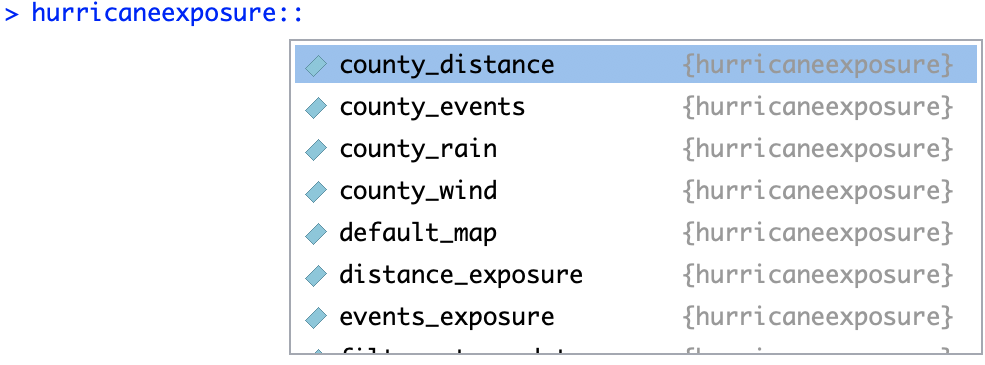
\includegraphics[width=13.68in]{images/tab_completion_example} \end{marginfigure}

\begin{Shaded}
\begin{Highlighting}[]
\KeywordTok{county_wind}\NormalTok{(}\DataTypeTok{counties =} \KeywordTok{c}\NormalTok{(}\StringTok{"36061"}\NormalTok{, }\StringTok{"25025"}\NormalTok{), }\DataTypeTok{start_year =} \DecValTok{1988}\NormalTok{, }
    \DataTypeTok{end_year =} \DecValTok{2015}\NormalTok{, }\DataTypeTok{wind_limit =} \FloatTok{17.5}\NormalTok{)}
\end{Highlighting}
\end{Shaded}

\begin{verbatim}
##       storm_id  fips vmax_sust vmax_gust
## 1     Bob-1991 25025  26.46639  39.43492
## 2     Bob-1991 36061  18.19559  27.11142
## 3  Bertha-1996 25025  29.64453  44.17035
## 4  Bertha-1996 36061  28.95496  43.14289
## 5   Floyd-1999 25025  24.46946  36.45949
## 6   Floyd-1999 36061  20.50178  30.54765
## 7   Hanna-2008 25025  18.36505  27.36392
## 8   Hanna-2008 36061  19.25390  28.68832
## 9   Irene-2011 36061  25.68553  38.27144
## 10  Sandy-2012 36061  21.99213  32.76827
##    sust_dur gust_dur closest_time_utc
## 1       210      570 1991-08-19 20:00
## 2         0      480 1991-08-19 15:00
## 3       240      525 1996-07-14 01:15
## 4       180      540 1996-07-13 19:45
## 5       345      750 1999-09-17 07:45
## 6        60      315 1999-09-17 00:15
## 7         0      150 2008-09-07 07:15
## 8         0      195 2008-09-07 01:45
## 9       165      510 2011-08-28 13:15
## 10      225      795 2012-10-30 00:30
##    storm_dist       local_time closest_date
## 1   27.042565 1991-08-19 16:00   1991-08-19
## 2  161.571830 1991-08-19 11:00   1991-08-19
## 3   38.177990 1996-07-13 21:15   1996-07-13
## 4   16.966013 1996-07-13 15:45   1996-07-13
## 5   51.254726 1999-09-17 03:45   1999-09-17
## 6   45.408483 1999-09-16 20:15   1999-09-16
## 7    6.202866 2008-09-07 03:15   2008-09-07
## 8   29.916672 2008-09-06 21:45   2008-09-06
## 9    5.796733 2011-08-28 09:15   2011-08-28
## 10 158.040788 2012-10-29 20:30   2012-10-29
\end{verbatim}

If you look up events based on flood events, you can instead run the
\texttt{county\_events} function:

\begin{Shaded}
\begin{Highlighting}[]
\KeywordTok{county_events}\NormalTok{(}\DataTypeTok{counties =} \KeywordTok{c}\NormalTok{(}\StringTok{"36061"}\NormalTok{, }\StringTok{"25025"}\NormalTok{), }
    \DataTypeTok{start_year =} \DecValTok{1996}\NormalTok{, }\DataTypeTok{end_year =} \DecValTok{2015}\NormalTok{, }\DataTypeTok{event_type =} \StringTok{"flood"}\NormalTok{)}
\end{Highlighting}
\end{Shaded}

\begin{verbatim}
##     fips     storm_id closest_time_utc
## 1  25025  Dennis-1999 1999-09-08 08:00
## 2  36061   Floyd-1999 1999-09-17 00:15
## 3  36061 Allison-2001 2001-06-17 14:15
## 4  36061 Frances-2004 2004-09-09 13:30
## 5  36061    Ivan-2004 2004-09-18 17:45
## 6  36061  Jeanne-2004 2004-09-29 06:30
## 7  36061   Beryl-2006 2006-07-20 22:15
## 8  36061   Barry-2007 2007-06-04 15:45
## 9  36061   Irene-2011 2011-08-28 13:15
## 10 25025   Sandy-2012 2012-10-29 22:00
## 11 25025  Andrea-2013 2013-06-08 11:30
## 12 36061  Andrea-2013 2013-06-08 06:45
##    storm_dist       local_time closest_date
## 1  390.047523 1999-09-08 04:00   1999-09-08
## 2   45.408483 1999-09-16 20:15   1999-09-16
## 3  158.909890 2001-06-17 10:15   2001-06-17
## 4  379.343696 2004-09-09 09:30   2004-09-09
## 5  311.346881 2004-09-18 13:45   2004-09-18
## 6  222.900157 2004-09-29 02:30   2004-09-29
## 7  207.358443 2006-07-20 18:15   2006-07-20
## 8  148.251718 2007-06-04 11:45   2007-06-04
## 9    5.796733 2011-08-28 09:15   2011-08-28
## 10 433.295980 2012-10-29 18:00   2012-10-29
## 11  45.412565 2013-06-08 07:30   2013-06-08
## 12  92.381282 2013-06-08 02:45   2013-06-08
\end{verbatim}

The \texttt{hurricaneexposure} package also has functions for mapping the exposure
data for specific storms. For example, to see the rainfall fro Hurricane Ivan in
2004, you can run:

\begin{Shaded}
\begin{Highlighting}[]
\KeywordTok{map_counties}\NormalTok{(}\DataTypeTok{storm =} \StringTok{"Ivan-2004"}\NormalTok{, }\DataTypeTok{metric =} \StringTok{"rainfall"}\NormalTok{)}
\end{Highlighting}
\end{Shaded}

\begin{figure*}
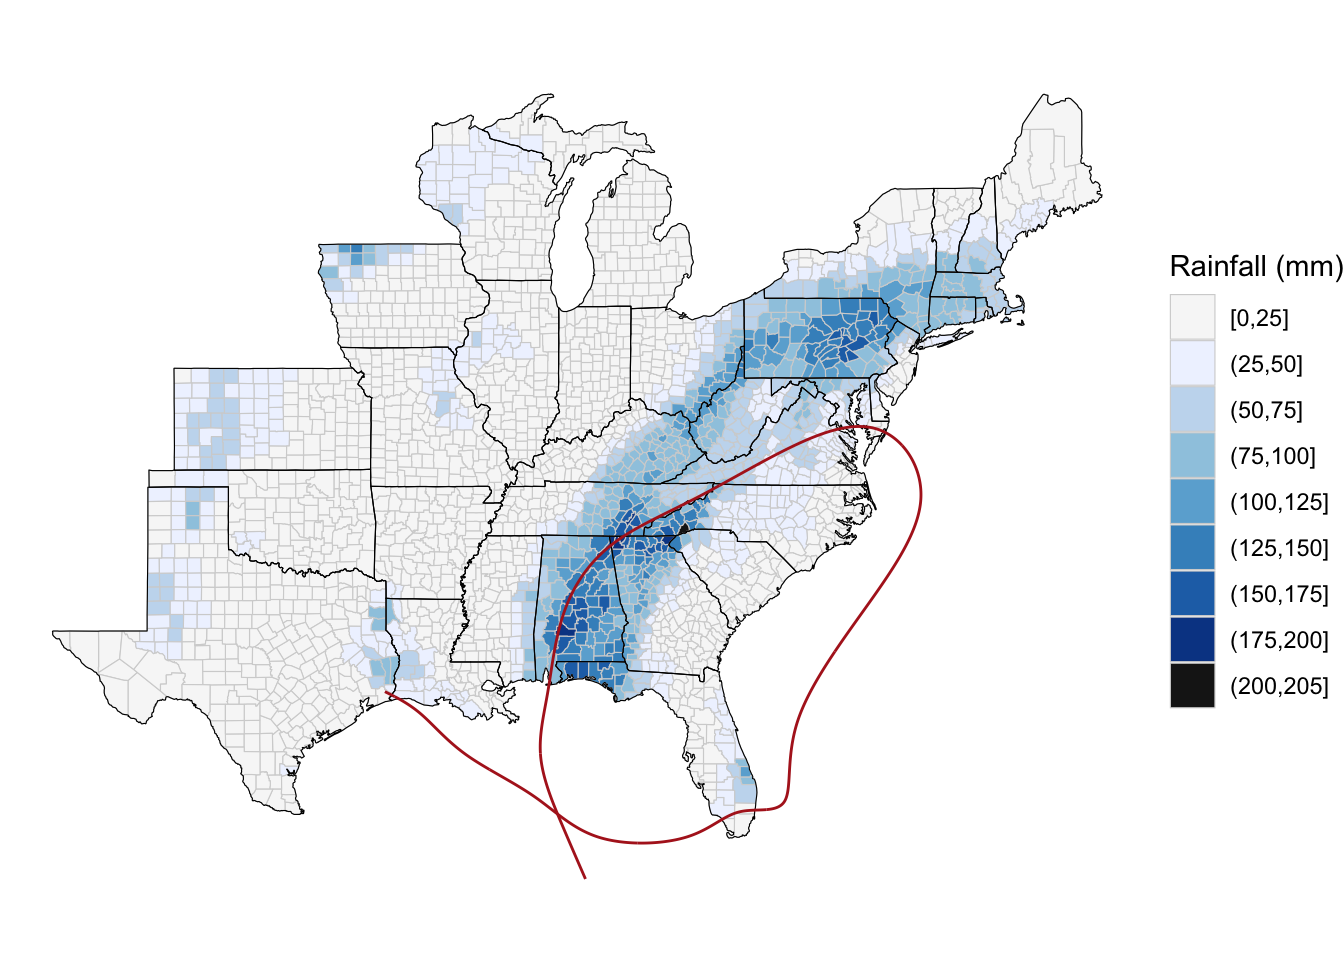
\includegraphics{columbia_env_health_files/figure-latex/unnamed-chunk-13-1} \end{figure*}

From this map, you can see that the rain from this storm extended into New
England, even after the storm looped back around to the east and south. This is
why New York City had heavy rainfall (and flooding) from this event, but not
tropical storm-level winds.

For more on the \texttt{hurricaneexposure} package, see \href{https://cran.r-project.org/web/packages/hurricaneexposure/vignettes/hurricaneexposure.html}{its vignette}.

\hypertarget{open-data-apis}{%
\section{Open data APIs}\label{open-data-apis}}

A range of environmental datasets are available online, especially through national agencies.
For example, NOAA provides various weather datasets, while USGS has data on water quality,

You can visit webpages hosted by these agencies where you can download the datasets you need.
However, this process can become tedious if you need lots of datasets, as may be the case for
large studies incorporating many cities. Further, downloading the datasets ``by hand'' is hard
to make reproducible, unless you meticiously write down all the steps you took as you visited
the website. This means that your process will be harder for you to repeat in the future
or for others to replicate.

A growing collection of R packages are now available that allow you to download datasets
available online directly from R. This means that you can write an R script for your data
collection, making this step both better documented and more reproducible.

One great example is the \texttt{tigris} package. This package lets you pull
spatial data into R directly from the US Census. To get spatial data for all the counties in
Florida, you can run:

\begin{Shaded}
\begin{Highlighting}[]
\KeywordTok{library}\NormalTok{(tigris)}
\NormalTok{fl_counties <-}\StringTok{ }\KeywordTok{counties}\NormalTok{(}\DataTypeTok{state =} \StringTok{"FL"}\NormalTok{, }\DataTypeTok{class =} \StringTok{"sf"}\NormalTok{)}
\end{Highlighting}
\end{Shaded}

Now you can plot this data with \texttt{ggplot}:

\begin{Shaded}
\begin{Highlighting}[]
\KeywordTok{library}\NormalTok{(ggplot2)}
\KeywordTok{ggplot}\NormalTok{() }\OperatorTok{+}\StringTok{ }\KeywordTok{geom_sf}\NormalTok{(}\DataTypeTok{data =}\NormalTok{ fl_counties, }\KeywordTok{aes}\NormalTok{(}\DataTypeTok{fill =}\NormalTok{ ALAND)) }\OperatorTok{+}\StringTok{ }
\StringTok{    }\KeywordTok{theme_bw}\NormalTok{() }\OperatorTok{+}\StringTok{ }\KeywordTok{scale_fill_viridis_c}\NormalTok{(}\DataTypeTok{name =} \StringTok{"Land area"}\NormalTok{, }
    \DataTypeTok{label =}\NormalTok{ scales}\OperatorTok{::}\NormalTok{scientific) }\OperatorTok{+}\StringTok{ }\KeywordTok{theme}\NormalTok{(}\DataTypeTok{axis.text =} \KeywordTok{element_blank}\NormalTok{(), }
    \DataTypeTok{axis.ticks =} \KeywordTok{element_blank}\NormalTok{())}
\end{Highlighting}
\end{Shaded}

\begin{center}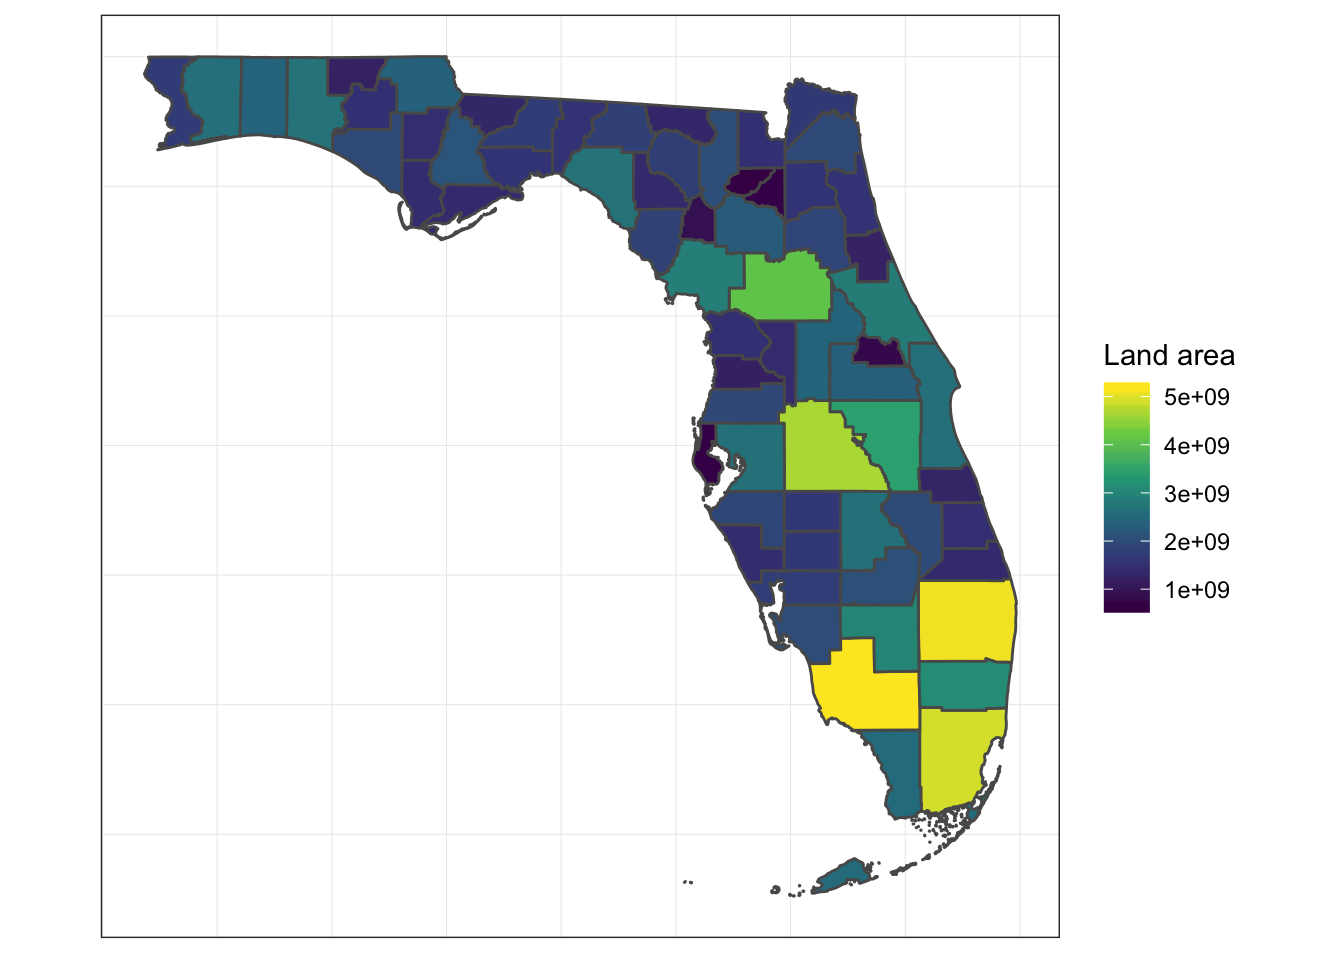
\includegraphics{columbia_env_health_files/figure-latex/unnamed-chunk-16-1} \end{center}

\hypertarget{learn-more-3}{%
\section{Learn more}\label{learn-more-3}}

One of the best places to explore R packages for accessing open data for science is
\href{https://ropensci.org/}{ROpenSci}.
Many of its packages facilitate access to databases of open data relevant to scientific
research that have web services. You can browse through its packages on
its \href{https://ropensci.org/packages/}{Packages page}. You may also want to
check its affiliated \href{https://joss.theoj.org/}{Journal of Open-Source Software}.
Authors of these packages will also sometimes publish associated articles in
\href{https://journal.r-project.org/}{The R Journal}, so it's worth browsing through
that occasionally.
Finally, Twitter is a great place ot keep an eye out for new packages, including
those that can help you collect data. Follow the ``\#rstats'' tag.

\bibliography{book.bib,packages.bib}



\end{document}
